% 02805 Social Graphs and Interactions — Final Project
% PNAS-style template (replace \author fields with your names)
\documentclass[9pt,twocolumn]{pnas-new}

\templatetype{pnasresearcharticle}

% Red placeholders for numbers that come from the updated notebook.
% After re-running project_analysis.ipynb, copy the values from the
% "PAPER STATISTICS" cell into every \tbd{...}, then delete this macro.
\usepackage{xcolor}
\newcommand{\tbd}[1]{\textcolor{red}{[#1]}}

\title{Culinary Communities: Network Structure and Linguistic Fingerprints in the Food.com Recipe Graph}

\author[a,1]{Ali Afif}
\author[a]{Group Member 2}
\author[a]{Group Member 3}

\affil[a]{Technical University of Denmark, DTU Compute, Kongens Lyngby, Denmark}

\leadauthor{Afif}

\significancestatement{%
Every dish is a network of ingredients. We show that the 500 most common ingredients on Food.com---one of the web's largest recipe platforms---organize into three culinary communities (Savory, Baking, and Asian) whose boundaries emerge only from which ingredients appear together, not from any explicit label. The communities are far stronger than in randomized networks with the same ingredient frequencies, they agree with the cuisine tags that users attach to recipes, and each one writes its cooking instructions with its own vocabulary. Yet recipes from all three communities are rated the same: culinary tradition shapes how we cook and talk about food, but not how much we say we like the result.%
}

\authorcontributions{%
A.A. built the network, ran community detection, and wrote the Results section. G.M.2 performed the TF-IDF and VADER sentiment analyses and wrote the Methods section. G.M.3 designed the figures, ran the validation checks, and wrote the Introduction and Discussion.%
}

\authordeclaration{The authors declare no competing interest.}

\equalauthors{\textsuperscript{1}To whom correspondence should be addressed. E-mail: aliafif@ymail.com}

\keywords{food networks | ingredient co-occurrence | community detection | natural language processing | recipe analysis}

\begin{abstract}
We analyse the Food.com dataset---87,313 recipes and over one million rated reviews---through the lens of network science and natural language processing. We build a weighted co-occurrence network of the 500 most frequent ingredients, linking two ingredients when they appear together in at least five recipes. Louvain community detection finds three culinary communities: Savory (320 ingredients), Baking (154), and Asian (26), with modularity $Q = 0.215$, against \tbd{$Q_\mathrm{null} = \ldots \pm \ldots$} for a strength-preserving configuration-model null. The partition is stable across random seeds and edge thresholds, and it aligns with the cuisine tags users attach to recipes (NMI $= 0.52$; permutation null $\approx 0$). A per-recipe TF-IDF analysis of cooking steps shows that each community has a distinctive vocabulary. Mean recipe ratings do not differ detectably between communities ($F = 2.76$, $p = 0.064$), and community membership explains only $0.006\%$ of rating variance. Betweenness centrality on this dense network is dominated by pantry staples---\textit{salt} alone lies on 92\% of sampled shortest paths---so we use the participation coefficient to identify the ingredients that genuinely connect communities.
\end{abstract}

\dates{This manuscript was submitted to 02805 Social Graphs and Interactions, DTU, Fall 2026.}

\begin{document}

\maketitle
\thispagestyle{firststyle}
\ifthenelse{\boolean{shortarticle}}{\ifthenelse{\boolean{singlecolumn}}{\abscontentformatted}{\abscontent}}{}

%% ---- INTRODUCTION ----
\section*{Introduction}

Food is a network. Every recipe is a set of ingredients that co-appear by design, and the structure of which ingredients appear together encodes culinary tradition, agricultural geography, and cultural exchange. Ahn et al.~\cite{ahn2011flavor} showed that Western cuisines tend to pair ingredients that share flavour compounds, while East Asian cuisines avoid such pairings---a signal visible in the network of ingredient co-occurrence. The Food.com dataset, originally collected by Majumder et al.~\cite{majumder2019generating} for personalized recipe generation, offers 231,637 recipes and over a million reviews, making it one of the richest publicly available cooking corpora.

We ask two related questions. First, \textit{what community structure emerges from ingredient co-occurrence, and does it correspond to recognizable culinary traditions?} Second, \textit{does community membership shape the language cooks use to write their recipes?} Prior work has used ingredient networks to recommend recipes and to find ingredient substitutes~\cite{teng2012recipe}, but the link between network communities and the language of cooking instructions has received little systematic attention.

We approach both questions with the toolkit of the course: Louvain community detection tested against a configuration-model null and checked for robustness to the edge threshold and to a disparity-filter backbone; external validation against cuisine tags (NMI); TF-IDF to extract community-specific vocabulary from cooking steps; VADER sentiment analysis validated against star ratings; and betweenness centrality and the participation coefficient to identify ingredients that sit between communities.

%% ---- RESULTS ----
\section*{Results}

\subsection*{The ingredient co-occurrence network}

We build a weighted undirected network whose nodes are the 500 most frequent ingredients (covering 79\% of all ingredient mentions) across the 87,313 recipes that have at least three rated reviews and at least two of these ingredients. Two ingredients are linked when they appear together in at least 5 recipes, and the edge is weighted by that count. The threshold removes 40,137 of the 87,468 observed ingredient pairs (46\%), leaving 500 nodes and 47,331 edges (density $0.379$, mean degree $189$). The network is very dense because pantry staples co-occur with almost everything: \textit{salt} appears in 40\% of recipes and has the largest weighted degree, followed by \textit{butter}, \textit{onion}, and \textit{sugar}.

\subsection*{Three culinary communities}

Louvain community detection~\cite{blondel2008fast} on the weighted network yields three communities (Figure~\ref{fig:network}): a large \textbf{Savory} community (320 ingredients; onion, olive oil, garlic, pepper, parmesan), a \textbf{Baking} community (154; salt, butter, sugar, eggs, flour, baking powder), and a small \textbf{Asian} community (26; soy sauce, honey, cornstarch, ginger, sesame oil, rice vinegar). Assigning each recipe to the community that holds most of its ingredients gives 54,308 Savory, 31,831 Baking, and 1,174 Asian recipes. The partition is stable: across 10 further random seeds, $Q$ ranges from \tbd{\ldots} to \tbd{\ldots} and the mean NMI with our main partition is \tbd{\ldots}.

The observed modularity is $Q = 0.215$. A dense network can show some modularity simply because a few ingredients are much more common than others, so we compare against a strength-preserving configuration model: we randomly re-pair all co-occurrences while every ingredient keeps its total co-occurrence count, and let Louvain find the best partition of each of 100 random networks. These reach only \tbd{$Q = \ldots \pm \ldots$} ($z = \ldots$, empirical $p \le \ldots$), so the community structure is not a by-product of ingredient frequencies.

The communities are also robust to how the network is built. Rebuilding it with thresholds of 1, 3, 10, and 20 co-occurrences, or extracting a disparity-filter backbone~\cite{serrano2009extracting} at $\alpha = 0.05$, gives partitions with NMI \tbd{\ldots--\ldots} relative to our main partition, and the Asian community stays together in \tbd{\ldots} of these variants.

As an external check, we compare each recipe's community with a cuisine label derived from its Food.com tags (Asian, Baking, or Savory; see Methods). On the 54,493 recipes that have such a tag, the normalized mutual information between community and tag is NMI $= 0.518$, against $4.6 \times 10^{-5}$ for 200 random permutations of the tags. The alignment is imperfect because many recipes mix traditions, but it shows that the communities found from co-occurrence alone match how users themselves categorize recipes.

\subsection*{Community-specific vocabulary in cooking steps}

Each community leaves a linguistic signature in how cooks write their recipe steps. We treat every recipe's step text as one document (up to 3,000 sampled recipes per community; all 1,174 for Asian), fit TF-IDF over all of them, and average the TF-IDF vectors within each community. A word is distinctive for a community when its average score there exceeds its average in the other two (Figure~\ref{fig:tfidf}).

\tbd{Describe the top words per community from the ``TF-IDF distinctive words'' line of the PAPER STATISTICS cell, e.g. Baking: \ldots; Savory: \ldots; Asian: \ldots.} The vocabulary split shows that communities defined purely by which ingredients co-occur also organize the language of cooking differently.

\subsection*{Hubs versus bridges}

We compute betweenness centrality~\cite{brandes2001faster} with edge length $1/w$, so that frequent co-occurrences are short paths, estimated from $k = 200$ randomly sampled source nodes (Figure~\ref{fig:betweenness}). On this dense network betweenness is extremely concentrated: \textit{salt} (Baking community) has normalized betweenness $0.917$, i.e. it lies on 92\% of the sampled shortest paths, followed by \textit{onion} ($0.201$), \textit{butter} ($0.136$), \textit{olive oil} ($0.108$), and \textit{sugar} ($0.104$). \textit{Soy sauce} ($0.027$) is the only Asian ingredient among the top 15. Because the heaviest edges all run through staples, betweenness here identifies pantry hubs rather than ingredients that connect distinct traditions.

To find genuine connectors we use the participation coefficient~\cite{guimera2005functional}, which measures how evenly an ingredient's co-occurrence weight is spread across the three communities ($0$ = all within its own community; maximum $2/3$). Among ingredients with above-median weighted degree, the strongest connectors are \tbd{\ldots}. Mean participation is \tbd{\ldots} for Savory, \tbd{\ldots} for Baking, and \tbd{\ldots} for Asian.

\subsection*{Community membership does not predict recipe ratings}

Despite these structural and linguistic differences, the three communities receive almost identical ratings: $4.658 \pm 0.375$ (Savory), $4.652 \pm 0.415$ (Baking), and $4.667 \pm 0.372$ (Asian). A one-way ANOVA gives $F = 2.76$, $p = 0.064$, and community membership explains $\eta^2 = 6 \times 10^{-5}$ of the variance in recipe ratings. With 87,313 recipes even a tiny difference would be detectable, so the non-significant result together with the negligible effect size means that any difference is too small to matter. At the ingredient level, neither degree ($r = -0.067$, $p = 0.14$) nor betweenness ($r = -0.017$, $p = 0.70$) correlates with the mean rating of the recipes an ingredient appears in.

Review text tells the same story. Mean VADER~\cite{hutto2014vader} compound scores are $0.782$ (Savory), $0.778$ (Baking), and $0.768$ (Asian) on 500 reviews per community ($F = 0.28$, $p = 0.76$). We validated VADER against star ratings on 5,000 sampled reviews (Methods): Cohen's $\kappa = 0.41$, with high accuracy on positive reviews but poor detection of the rare negative ones (precision $0.39$, recall $0.46$ on 102 negative reviews), consistent with the strong positive skew of the platform (76\% of ratings are five stars).

%% ---- DISCUSSION ----
\section*{Discussion}

The ingredient space of Food.com is not flat. It partitions into three communities that are much stronger than in randomized networks with the same ingredient frequencies, survive changes to how the network is built, correspond to the cuisine tags users assign, and come with their own cooking vocabulary. Network structure and language are therefore two views of the same culinary traditions.

A methodological lesson concerns centrality. In a network this dense, betweenness does not find cultural bridges: it finds \textit{salt}. The shortest weighted paths between almost any two ingredients pass through the few staples that co-occur with everything. Asking which ingredients spread their links across communities (the participation coefficient) is a more direct way to find connectors, and it gives a different answer from asking which ingredients are most central.

Several limitations bear noting. The edge threshold of 5 co-occurrences is a choice; we show that the communities are robust to it, but it still prunes rare pairings that may carry culturally specific signal, particularly for cuisines with few representatives among the 500 most common ingredients (Middle Eastern, Indian, Latin American). The Asian community is small (26 ingredients, 1,174 recipes) because soy-based ingredients are relatively rare on a predominantly English-language platform. Assigning each recipe to the community holding most of its ingredients may misclassify fusion dishes. The cuisine labels used for validation come from a hand-picked list of tags. And VADER's moderate agreement with star ratings ($\kappa = 0.41$), driven by poor detection of negative reviews, limits what can be concluded from review sentiment.

Finally, the absence of a rating difference should be read carefully. It does not show that all traditions are ``equally good''; it shows that, on a platform where 76\% of ratings are five stars, users rate recipes from all three communities equally highly. Culinary tradition shapes how people cook and how they write about cooking, but not how they rate the result.

%% ---- METHODS ----
\section*{Methods}

\paragraph{Data.}
We use the publicly available Food.com Recipes and Interactions dataset~\cite{majumder2019generating} (231,637 recipes). We discard interactions with a rating of 0, which mark reviews without a rating, leaving 1,071,520 rated reviews. We keep recipes with at least 3 rated reviews (90,437) and, after filtering ingredients to the 500 most frequent ones, recipes with at least two such ingredients (87,313).

\paragraph{Network construction.}
Ingredients are parsed from their string-list representation. For every pair of the top-500 ingredients that co-appear in a recipe, we increment an edge counter. Pairs with fewer than 5 co-occurrences are pruned (40,137 of 87,468 pairs). All 500 nodes remain in a single connected component. Edge weight equals co-occurrence count.

\paragraph{Community detection.}
We run Louvain~\cite{blondel2008fast} (python-louvain) on the weighted network with random seed 42 and report this partition. To check stability we rerun it with 10 other seeds and compare each partition with the main one using NMI. Communities are named by their dominant ingredients: the community containing soy sauce or sesame oil is Asian; the one containing sugar, flour, and baking powder is Baking; the remaining one is Savory.

\paragraph{Null model.}
We use a strength-preserving configuration model~\cite{maslov2002specificity,newman2004finding}, the weighted analogue of a degree-preserving shuffle. Each edge of weight $w$ is treated as $w$ co-occurrence units. We split every unit into two stubs, shuffle all stubs, and pair them up again, discarding self-pairs. Each ingredient keeps its strength while its partners are randomized. We run Louvain on 100 such networks and report the mean and standard deviation of their modularity, the $z$-score of the observed $Q$, and the empirical $p$-value $(1 + \#\{Q_\mathrm{null} \ge Q\})/(1 + 100)$.

\paragraph{Robustness.}
We rebuild the network with thresholds of 1, 3, 10, and 20, and extract a disparity-filter backbone~\cite{serrano2009extracting} from the unthresholded network: an edge is kept if $(1 - w_{ij}/s_i)^{k_i - 1} < 0.05$ for at least one endpoint $i$, where $s_i$ is the strength and $k_i$ the degree of $i$. For each variant we run Louvain (best of 5 seeds), compute the NMI with the main partition on shared nodes, and record the largest fraction of the main Asian community's ingredients that end up in a single community.

\paragraph{External validation (NMI).}
Each recipe is assigned to its plurality community, i.e. the community containing most of its top-500 ingredients. Recipes are labelled from their Food.com tags, checked in this order: any of \{asian, chinese, japanese, korean, thai, vietnamese\} is Asian; any of \{baking, cake(s), cookie(s), dessert(s), pastry, muffin(s), pie(s), bread\} is Baking; any of \{main-dish, chicken, beef, pasta, soup, stew, meat, pork, seafood\} is Savory. Recipes without any of these tags are excluded. We compute NMI between community and label and compare with 200 random permutations of the labels.

\paragraph{TF-IDF linguistic analysis.}
We sample up to 3,000 recipes per community and treat each recipe's concatenated step text as one document. We remove English stop words and 38 generic cooking words (verbs such as \textit{add}, \textit{stir}, \textit{mix}, \textit{heat}; units such as \textit{cup}, \textit{minutes}; and utensils such as \textit{bowl}, \textit{pan}, \textit{oven}) before fitting a TF-IDF vectorizer (unigrams, sublinear term frequency, words in at least 5 recipes, at most 8,000 features). We average the TF-IDF vectors within each community and rank words by the difference between their community mean and their mean in the other two communities.

\paragraph{Centrality.}
Betweenness centrality~\cite{brandes2001faster} is computed with edge length $1/w_{ij}$ and estimated from $k = 200$ randomly sampled source nodes (seed 42). The participation coefficient~\cite{guimera2005functional} of ingredient $i$ is $P_i = 1 - \sum_c (s_{i,c}/s_i)^2$, where $s_{i,c}$ is the total weight of $i$'s edges into community $c$.

\paragraph{Ratings.}
We compare mean recipe ratings across communities with a one-way ANOVA and report $\eta^2$ (between-community sum of squares divided by total sum of squares). For each ingredient with at least 20 recipes we correlate its degree and betweenness with the mean rating of its recipes (Pearson), and compare the degree correlation with 1,000 shuffles of the ratings.

\paragraph{Sentiment analysis.}
We apply VADER~\cite{hutto2014vader} to reviews longer than 20 characters. For validation we sample 5,000 such reviews and treat ratings $\geq 4$ as positive and $\leq 2$ as negative, and VADER compound scores $\geq 0.05$ as positive and $\leq -0.05$ as negative. Dropping three-star reviews and VADER-neutral reviews leaves 4,765 pairs, on which we compute Cohen's $\kappa$. Community differences in sentiment are tested with a one-way ANOVA on 500 reviews per community.

\paragraph{Code and data.}
All analyses are in the accompanying notebook \texttt{project\_analysis.ipynb}.

%% ---- REFERENCES ----
\bibliography{references}

%% ---- FIGURES ----
\begin{figure}[htb]
\centering
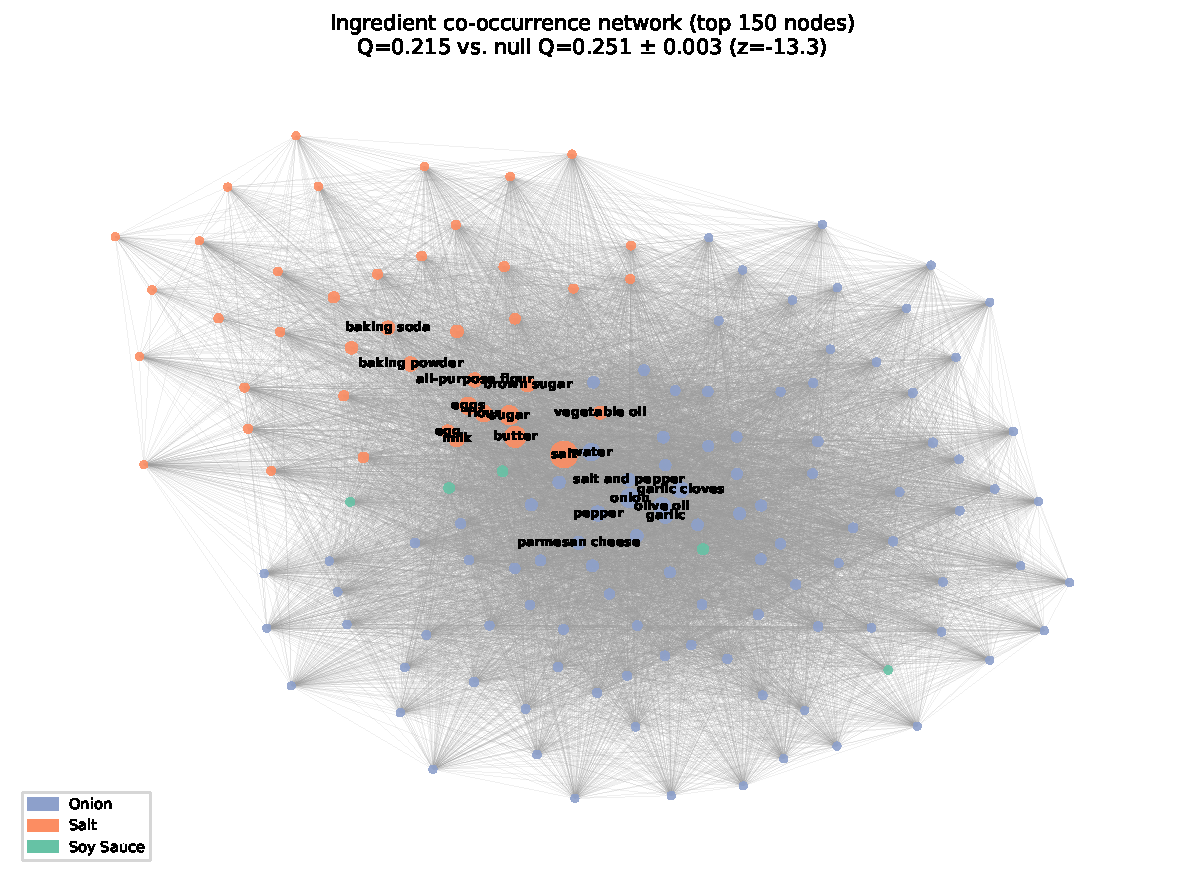
\includegraphics[width=\linewidth]{fig1_network.pdf}
\caption{\textbf{Ingredient co-occurrence network.} The 120 ingredients with the highest weighted degree are shown; node size scales with weighted degree, and the 20 largest nodes are labelled. Colours denote Louvain communities: Savory (blue, 320 ingredients), Baking (orange, 154), and Asian (green, 26). Modularity $Q = 0.215$, compared with \tbd{$\ldots \pm \ldots$} for Louvain on 100 strength-preserving random networks.}
\label{fig:network}
\end{figure}

\begin{figure}[htb]
\centering
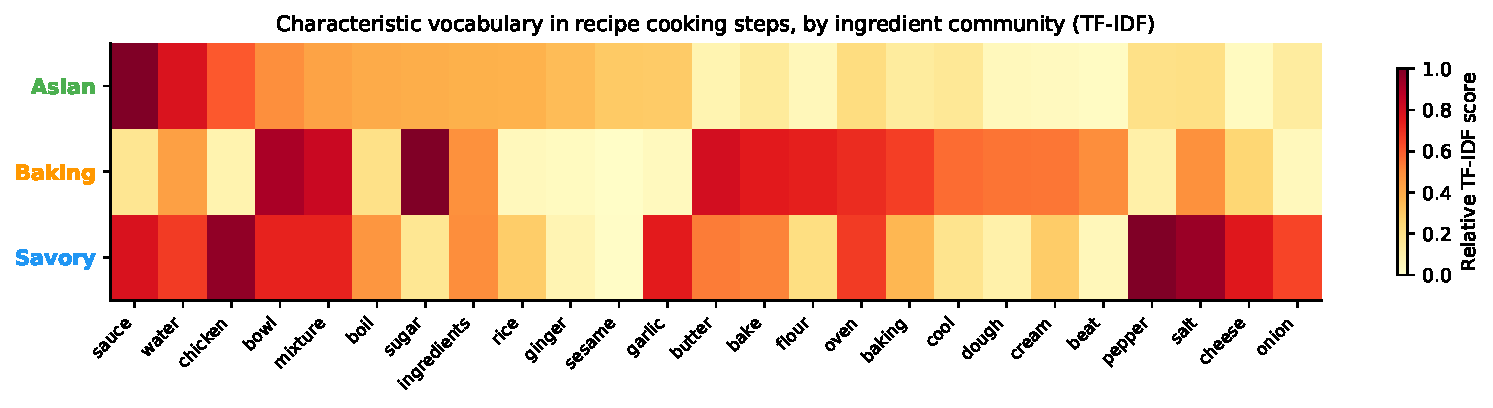
\includegraphics[width=\linewidth]{fig2_tfidf.pdf}
\caption{\textbf{Linguistic fingerprints of culinary communities.} Mean per-recipe TF-IDF of cooking-step text for the 10 most distinctive words of each community (words whose mean score in that community most exceeds their mean in the other two). Each row is normalized to its maximum. Up to 3,000 recipes per community (all 1,174 Asian recipes); English stop words and generic cooking words (\textit{add}, \textit{stir}, \textit{mix}, \textit{heat}, units, utensils) were removed before fitting.}
\label{fig:tfidf}
\end{figure}

\begin{figure}[htb]
\centering
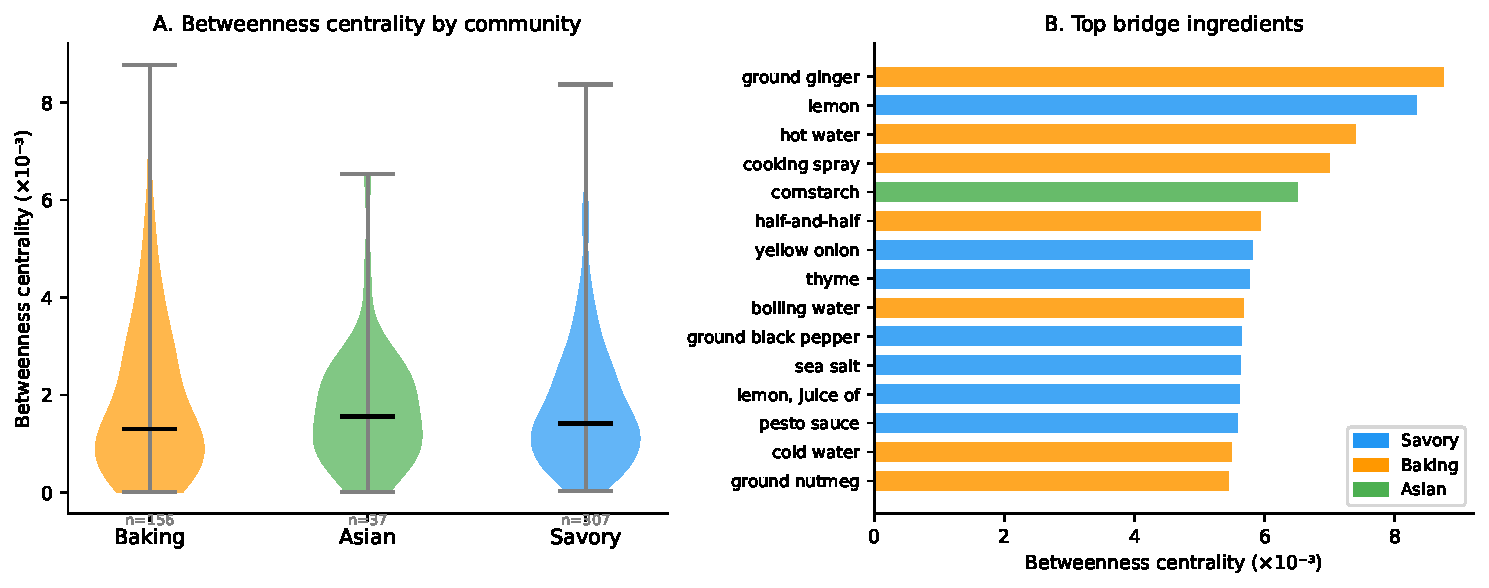
\includegraphics[width=\linewidth]{fig3_betweenness.pdf}
\caption{\textbf{Betweenness centrality is dominated by pantry staples.} \textbf{(A)} Distribution of betweenness centrality ($\times 10^{-3}$) across ingredients in each community; almost all ingredients have betweenness close to zero, and the long Baking tail is a single ingredient, \textit{salt}. \textbf{(B)} The 15 ingredients with the highest betweenness. \textit{Salt} ($917 \times 10^{-3}$) lies on most sampled shortest paths, followed by \textit{onion}, \textit{butter}, \textit{olive oil}, and \textit{sugar}; \textit{soy sauce} is the only Asian ingredient in the top 15. Edge length is $1/w$, estimated from 200 sampled source nodes.}
\label{fig:betweenness}
\end{figure}

\end{document}
